\documentclass{article}
\usepackage{graphicx} % This line is necessary to use \includegraphics
% if you need to pass options to natbib, use, e.g.:
%     \PassOptionsToPackage{numbers, compress}{natbib}
% before loading neurips_2019

% ready for submission
% \usepackage{neurips_2019}

% to compile a preprint version, e.g., for submission to arXiv, add add the
% [preprint] option:
%     \usepackage[preprint]{neurips_2019}

% to compile a camera-ready version, add the [final] option, e.g.:
% \usepackage[]{neurips_2019}
\usepackage{project_440_550}

% to avoid loading the natbib package, add option nonatbib:
%     \usepackage[nonatbib]{neurips_2019}

\usepackage[utf8]{inputenc} % allow utf-8 input
\usepackage[T1]{fontenc}    % use 8-bit T1 fonts
\usepackage{hyperref}       % hyperlinks
\usepackage{cleveref}
\usepackage{url}            % simple URL typesetting
\usepackage{booktabs}       % professional-quality tables
\usepackage{amsfonts}       % blackboard math symbols
\usepackage{nicefrac}       % compact symbols for 1/2, etc.
\usepackage{microtype}      % microtypography

\usepackage[dvipsnames]{xcolor}
\usepackage[normalem]{ulem}
\newif{\ifhidecomments}


\title{[Re] Diffusion-Based Adversarial Sample Generation for Improved Stealthiness and Controllability}

% The \author macro works with any number of authors. There are two commands
% used to separate the names and addresses of multiple authors: \And and \AND.
%
% Using \And between authors leaves it to LaTeX to determine where to break the
% lines. Using \AND forces a line break at that point. So, if LaTeX puts 3 of 4
% authors names on the first line, and the last on the second line, try using
% \AND instead of \And before the third author name.


\author{%
  William Kang,
  \\
  \texttt{wkang01@student.ubc.ca}
  \And
  Christina Yang\\
  \texttt{chryang@student.ubc.ca}
}

\begin{document}

\maketitle

\begin{abstract}
  We are doing a reproducibility report based on the paper "Diffusion-Based Adversarial Sample Generation for Improved Stealthiness and Controllability" by Haotian Xue, Alexandre Araujo, Bin Hu, Yongxin Chen. Their Github Repo is here: \url{https://github.com/xavihart/Diff-PGD/tree/main}.

  The paper uses a novel framework to generate adversarial samples. They use a gradient based method guided by a pre-trained diffusion model to try to generate images that appear realistic to the human eye, can fool a wide range of models, and is easy to control how certain regions are modified.

  In particular, we are evaluating the claims that Diff-PGD outperform baseline methods such as PGD, AdvPatch, and AdvCam in physical-world attacks and style-based attacks specifically.
  Finally, we are evaluating the claim that Diff-PGD generates adversarial samples with higher stealthiness.
\end{abstract}


% \section*{\centering Reproducibility Summary}

% \textit{Template and style guide to \href{https://paperswithcode.com/rc2020}{ML Reproducibility Challenge 2020}. The following section of Reproducibility Summary is \textbf{mandatory}. This summary \textbf{must fit} in the first page, no exception will be allowed. When submitting your report in OpenReview, copy the entire summary and paste it in the abstract input field, where the sections must be separated with a blank line.
% }

% \subsection*{Scope of Reproducibility}

% State the main claim(s) of the original paper you are trying to reproduce (typically the main claim(s) of the paper).
% This is meant to place the work in context, and to tell a reader the objective of the reproduction.

% \subsection*{Methodology}

% Briefly describe what you did and which resources you used. For example, did you use author's code? Did you re-implement parts of the pipeline? You can also use this space to list the hardware used, and the total budget (e.g. GPU hours) for the experiments.

% \subsection*{Results}

% Start with your overall conclusion --- where did your results reproduce the original paper, and where did your results differ? Be specific and use precise language, e.g. "we reproduced the accuracy to within 1\% of reported value, which supports the paper's conclusion that it outperforms the baselines". Getting exactly the same number is in most cases infeasible, so you'll need to use your judgement to decide if your results support the original claim of the paper.

% \subsection*{What was easy}

% Describe which parts of your reproduction study were easy. For example, was it easy to run the author's code, or easy to re-implement their method based on the description in the paper? The goal of this section is to summarize to a reader which parts of the original paper they could easily apply to their problem.

% \subsection*{What was difficult}

% Describe which parts of your reproduction study were difficult or took much more time than you expected. Perhaps the data was not available and you couldn't verify some experiments, or the author's code was broken and had to be debugged first. Or, perhaps some experiments just take too much time/resources to run and you couldn't verify them. The purpose of this section is to indicate to the reader which parts of the original paper are either difficult to re-use, or require a significant amount of work and resources to verify.

% \subsection*{Communication with original authors}

% Briefly describe how much contact you had with the original authors (if any).
% \newpage
\textit{\textbf{The following section formatting is \textbf{optional}, you can also define sections as you deem fit.
\\
Focus on what future researchers or practitioners would find useful for reproducing or building upon the paper you choose.}}
\section{Introduction}
% A few sentences placing the work in high-level context. Limit it to a few paragraphs at most; your report is on reproducing a piece of work, you don’t have to motivate that work.

Neural networks are remarkably good at tasks such as image classification. However, they are susceptible to attacks that perturb images in subtle ways, causing the model to classify one image as something else entirely.
These perturbed samples are called adversarial samples, and are a major security concern for systems that use neural networks.
There are various types of adversarial attacks, including global attacks, which perturb any part of the image, regional attacks, which change a specified region of an image, style-based attacks, which change an image region based on a reference image, and physical world attacks, which generates images you can print out and place on a physical object which cause the physical object to be misclassified by an image classifier.

The authors of the original paper propose a new method for generating adversarial models, that uses an off-the-shelf diffusion model to help guide the generation of the perturbations in the image, called Diff-PGD.
This method aims to create adversarial samples that are more realistic, and harder to detect by the human eye, compared to baseline methods, and can be applied to various types of attacks, such as digital attacks, physical-world attacks, and style-based attacks.\\



\section{Scope of reproducibility}
\label{sec:claims}

% Introduce the specific setting or problem addressed in this work, and list the main claims from the original paper. Think of this as writing out the main contributions of the original paper. Each claim should be relatively concise; some papers may not clearly list their claims, and one must formulate them in terms of the presented experiments. (For those familiar, these claims are roughly the scientific hypotheses evaluated in the original work.)

% A claim should be something that can be supported or rejected by your data. An example is, ``Finetuning pretrained BERT on dataset X will have higher accuracy than an LSTM trained with GloVe embeddings.''
% This is concise, and is something that can be supported by experiments.
% An example of a claim that is too vague, which can't be supported by experiments, is ``Contextual embedding models have shown strong performance on a number of tasks. We will run experiments evaluating two types of contextual embedding models on datasets X, Y, and Z."

% This section roughly tells a reader what to expect in the rest of the report. Clearly itemize the claims you are testing:

The main claims from the original paper are as follows:
\begin{enumerate}
    % \item Diffusion-Based Projected Gradient Descent (Diff-PGD) generates realistic adversarial samples
    \item Diff-PGD can be applied to specific tasks such as digital attacks, physical-world attacks, and style-based attacks, outperforming baseline methods such as PGD, AdvPatch, and AdvCam.
    \item Diff-PGD is more stable and controllable compared to existing methods for generating natural-style adversarial samples.
    % \item The samples generated using Diff-PGD have better transferability and anti-purification power than traditional gradient-based methods.
    \item Diff-PGD surpasses the original PGD in Transferability and Purification power
    \item Diff-PGD generates adversarial samples with higher stealthiness
    % \item Diff-PGD generates images that are more stealthy compared to PGD-generated samples for digital attacks.
    % \item Diff-rPGD generates images that are more stealthy compared to rPGD-generated samples for digital attacks.
\end{enumerate}

We will be exploring the first claim in regards to physical-world~\ref{sec:results} and style-based attacks~\ref{sec:results} specifically.

% Each experiment in Section~\ref{sec:results} will support (at least) one of these claims, so a reader of your report should be able to separately understand the \emph{claims} and the \emph{evidence} that supports them.

%\jdcomment{To organizers: I asked my students to connect the main claims and the experiments that supported them. For example, in this list above they could have ``Claim 1, which is supported by Experiment 1 in Figure 1.'' The benefit was that this caused the students to think about what their experiments were showing (as opposed to blindly rerunning each experiment and not considering how it fit into the overall story), but honestly it seemed hard for the students to understand what I was asking for.}

\section{Methodology}


% Explain your approach - did you use the author's code, or did you aim to re-implement the approach from the description in the paper? Summarize the resources (code, documentation, GPUs) that you used.

\subsection{Model descriptions}
We used ResNet-50, ResNet-101, ResNet-18, Wide-ResNet-50, and Wide-ResNet-101 to classify images. The parameter `weights` was set to the default weight for each model.

\subsection{Datasets}
% For each dataset include 1) relevant statistics such as the number of examples and label distributions, 2) details of train / dev / test splits, 3) an explanation of any preprocessing done, and 4) a link to download the data (if available).

The original paper used ImageNet, but due to limitations in compute and memory, we used a smaller subset of ImageNet with 1000 samples: \url{https://www.kaggle.com/datasets/ifigotin/imagenetmini-1000}

% \subsection{Hyperparameters}
% Describe how the hyperparameter values were set. If there was a hyperparameter search done, be sure to include the range of hyperparameters searched over, the method used to search (e.g. manual search, random search, Bayesian optimization, etc.), and the best hyperparameters found. Include the number of total experiments (e.g. hyperparameter trials). You can also include all results from that search (not just the best-found results).



\subsection{Experimental setup and code}
% Include a description of how the experiments were set up that's clear enough a reader could replicate the setup.
% Include a description of the specific measure used to evaluate the experiments (e.g. accuracy, precision@K, BLEU score, etc.).
% Provide a link to your code.

We used the authors' code, however, since not all parts of the authors' code have been released, we wrote our own code to evaluate a lot of the experiments.
We also expanded on some of the authors' experiments with our own code, and reduced the number of iterations in a number of cases, due to time and compute constraints.
We also added our own code for evaluating the success rates of the authors' code.\\
% We ran the code given by the authors.
% We copied the hyperparameter setup of the authors for the most part, but reduced the number of iterations in many cases, and also added our own code for evaluating the success rates of the authors' code.\\

\subsubsection{Success Attack Rate}
We wrote our own code to test success rate in \url{attack_global.py}.
We used the same hyperparameters for running Attack\_Global as the authors, except that we chose to use skip=20, to use 78 images per iteration to test success rate.
If the adversarial sample caused the model to classify the image as anything other than it's original classification, we considered it a successful attack.\\

\subsubsection{Physical-World Attacks}
% We first tried the one of the attacks created by the authors, which was a computer-mouse.\\
We tried our own physical world attack using an image patch of a digitally drawn panda head and a laptop as our target object.\\

We use a Galaxy A53 5G to take images from the real world and used a MP C4505ex Color Laser Multifunction Printer to print the images in color.\\

Due to time and compute constraints, we chose to run 1500 iterations for each method instead of 4000 like the original model. We chose 1500 because after running one of the original paper's physical world attacks, the loss converged after around 1000 iterations.

We took the adversarial samples generated using each method (AdvCam, AdvPatch, and Diff-PDG) and stuck them on a laptop.
We then took multiple pictures of the laptop with the sample on top, with the sample in various different locations and rotations, and tested for success rate on the these photos by classifying them with ResNet-50.
% We tested for Success Attack Rate of Diff-PGD using 250 uniformly sampled images from our dataset. (See figure ...)\\
% The code for the figure in the paper was not provided, so we created our own code to generate the figure.\\

% We also need to generate anti-purification table from paper, but I'm not sure how to generate this.

% Transferability: Figure 6b+6c\\
% We also test the success rate attacking adversarially trained ResNet-50
\subsubsection{Style-Based Attacks}

\subsection{Computational requirements}
We ran it on either CPU or MPS. For used MPS for style-based attacks and global attacks, and CPU for physical-world attacks.
For each model, include a measure of the average runtime (e.g. average time to predict labels for a given validation set with a particular batch size).\\

Global attack success rate took between 5-6 hours to run, while physical-world attacks for one target object and patch took around 1-2 days to run for 1500 iterations.\\

Style-based attack took around 15s per iteration to run.\\
% For each experiment, include the total computational requirements (e.g. the total GPU hours spent).
% (Note: you'll likely have to record this as you run your experiments, so it's better to think about it ahead of time). Generally, consider the perspective of a reader who wants to use the approach described in the paper --- list what they would find useful.

\section{Results}
\label{sec:results}
Start with a high-level overview of your results. Do your results support the main claims of the original paper? Keep this section as factual and precise as possible, reserve your judgement and discussion points for the next "Discussion" section.
% \begin{center}
%   Original paper results
%   \begin{tabular}{ l c c c c r }
%     \hline
%     \textbf{Sample} & \textbf{(+P)ResNet50} & \textbf{(+P)ResNet101} & \textbf{(+P)ResNet18} & \textbf{(+P)WRN50} & \textbf{(+P)WRN101} \\ \hline
%     $x_{PGD}$ & 0.35 & 0.18 & 0.26 & 0.20 & 0.17 \\
%     $x_{n}$ (Ours) & 0.35 & 0.18 & 0.26 & 0.20 & 0.17 \\
%     $x_{n}^0$ (Ours) & 0.35 & 0.18 & 0.26 & 0.20 & 0.17 \\
%     \hline
%   \end{tabular}
% \end{center}



\subsection{Results reproducing original paper}
For each experiment, say 1) which claim in Section~\ref{sec:claims} it supports, and 2) if it successfully reproduced the associated experiment in the original paper.
For example, an experiment training and evaluating a model on a dataset may support a claim that that model outperforms some baseline.
Logically group related results into sections.

% skip=20

\subsubsection{Attack success rate}
\begin{figure}
  \centering
  % The next line would normally be \includegraphics instead.
  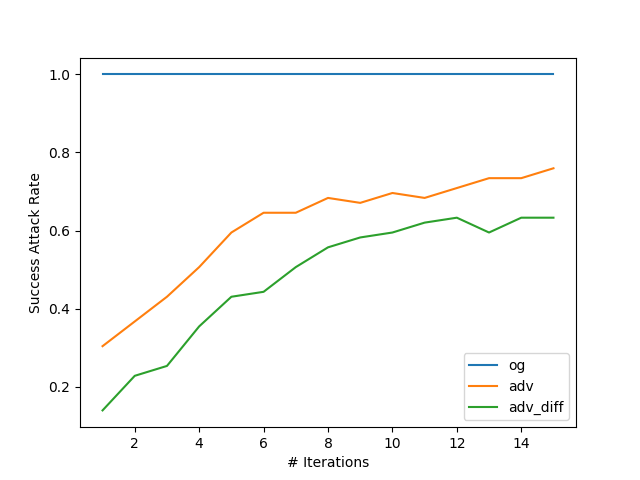
\includegraphics[scale=0.8]{figures/attack_global_gradpass_success_rate.png}

  \caption{
    Blue line is success rate of classifying an image not attacked.
    Orange line is success rate of causing a different classification with Diff-PGD.
    Green line is success rate of causing a different classification with Diff-PGD after applying sdedit at the end (purification???).
  }
  \label{fig:attack_success_rate}
\end{figure}

We got a very different result for success rate from that of the original paper (\cref{fig:attack_success_rate}). In the original paper, the success rate of all of the attacks reached 100\% after 5 iterations.
However, in our case the success rate reached only 60\%-80\% after 15 iterations.\\

\subsubsection{Physical-World Attacks}
None of the adversarial samples generated by AdvCam, AdvPatch, or Diff-PGD were able to perturb the classification of the image. This was likely due to the fact that we did not adjust the scale properly. This likely means that hyperparameter tuning is very important for physical-world attacks.\\

Because of this, we failed to support or reject the claim that Diff-PGD can be applied to physical-world attacks. However, from the samples generated, the Diff-PGD samples looked less stealthy and more perturbed than those of AdvCam and AdvPatch, which does not support the paper's claim that Diff-PGD generates samples with higher stealthiness.
However this is likely unimportant in regards to physical-world samples, since the samples generated through every method were quite obviously perturbed.\\

\begin{figure}
  \centering
  % The next line would normally be \includegraphics instead.
  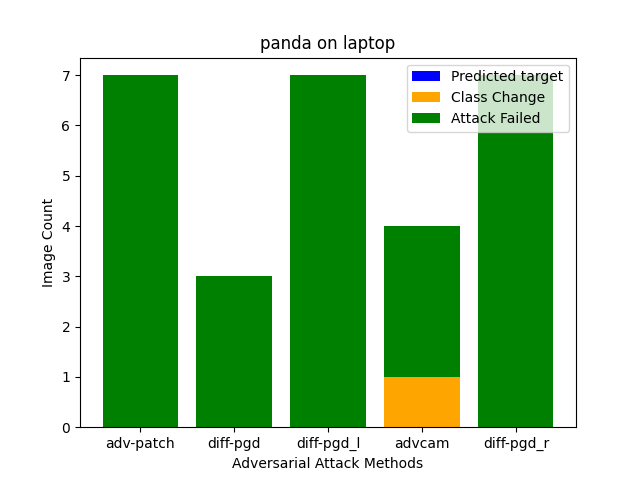
\includegraphics[scale=0.42]{figures/physical_panda_on_laptop_success_rate.png}
  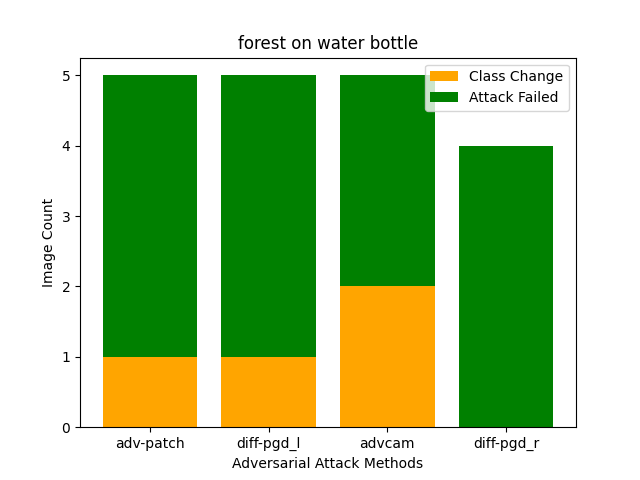
\includegraphics[scale=0.42]{figures/physical_forest_on_water_bottle_success_rate.png}

  \caption{
    Blue line is the number of images that were classified correctly as the target label.
    Orange line is the number of images that had a different classification with ResNet-50, but that is not the target class.
    Green line is the number of images whose classifications were one of the following:
    'notebook, notebook computer' and 'iPod' for panda on laptop, and
    'rain barrel', 'lighter, light, igniter, ignitor', 'pill bottle', 'hand blower, blow dryer, blow drier, hair dryer and hair drier' for forest on water bottle.
    These are the classes ResNet-50 gave to images with no adversarial sample (the original image on target object or no image on target object), or classes that we decided had the same meaning as the target object class (ie. laptop vs. notebook computer)
  }
  \label{fig:attack_success_rate}
\end{figure}

% We used a laptop as our target object and printed out an image of a laptop. We then stuck the image on a laptop and classified it using all 5 classifiers. We found that the attack was successful for all 5 classifiers. This supports the claim that Diff-PGD can be applied to physical-world attacks.

% We present the result of physical world attacks using adversarial patches
% generated using Diff-PGD in the main paper. In order to show that the adversarial patches are robust
% to camera views, we show more images taken from different camera views in Figure 16. For the
% two cases: computer mouse (untargeted) and back bag (targeted to Yorkshire Terrier), we randomly
% sample ten other camera views. The results show that the adversarial patches are robust both for
% targeted settings and untargeted settings. For targteted settings, our adversarial patch can fool the
% network to predict back bag as terriers, and for untargeted settings, the adversarial patch misleads the
% network to predict computer mouse as artichoke

\subsubsection{Style-Based Attacks}

\subsection{Experiment Setup}
For each iteration, we take a random base image from the test set of the ImageNetMini dataset.
Then for each image we compare the success rate for creating adversarial samples under 3 different attacks:
\begin{enumerate}
  \item Style-based attack with a different target image from ImageNetMini. Along with a mask generated based on the base image
  \item The same as the above, except no mask is applied.
  \item Global attack which has no target image and no mask
\end{enumerate}

\begin{figure}
  \centering
  % The next line would normally be \includegraphics instead.
  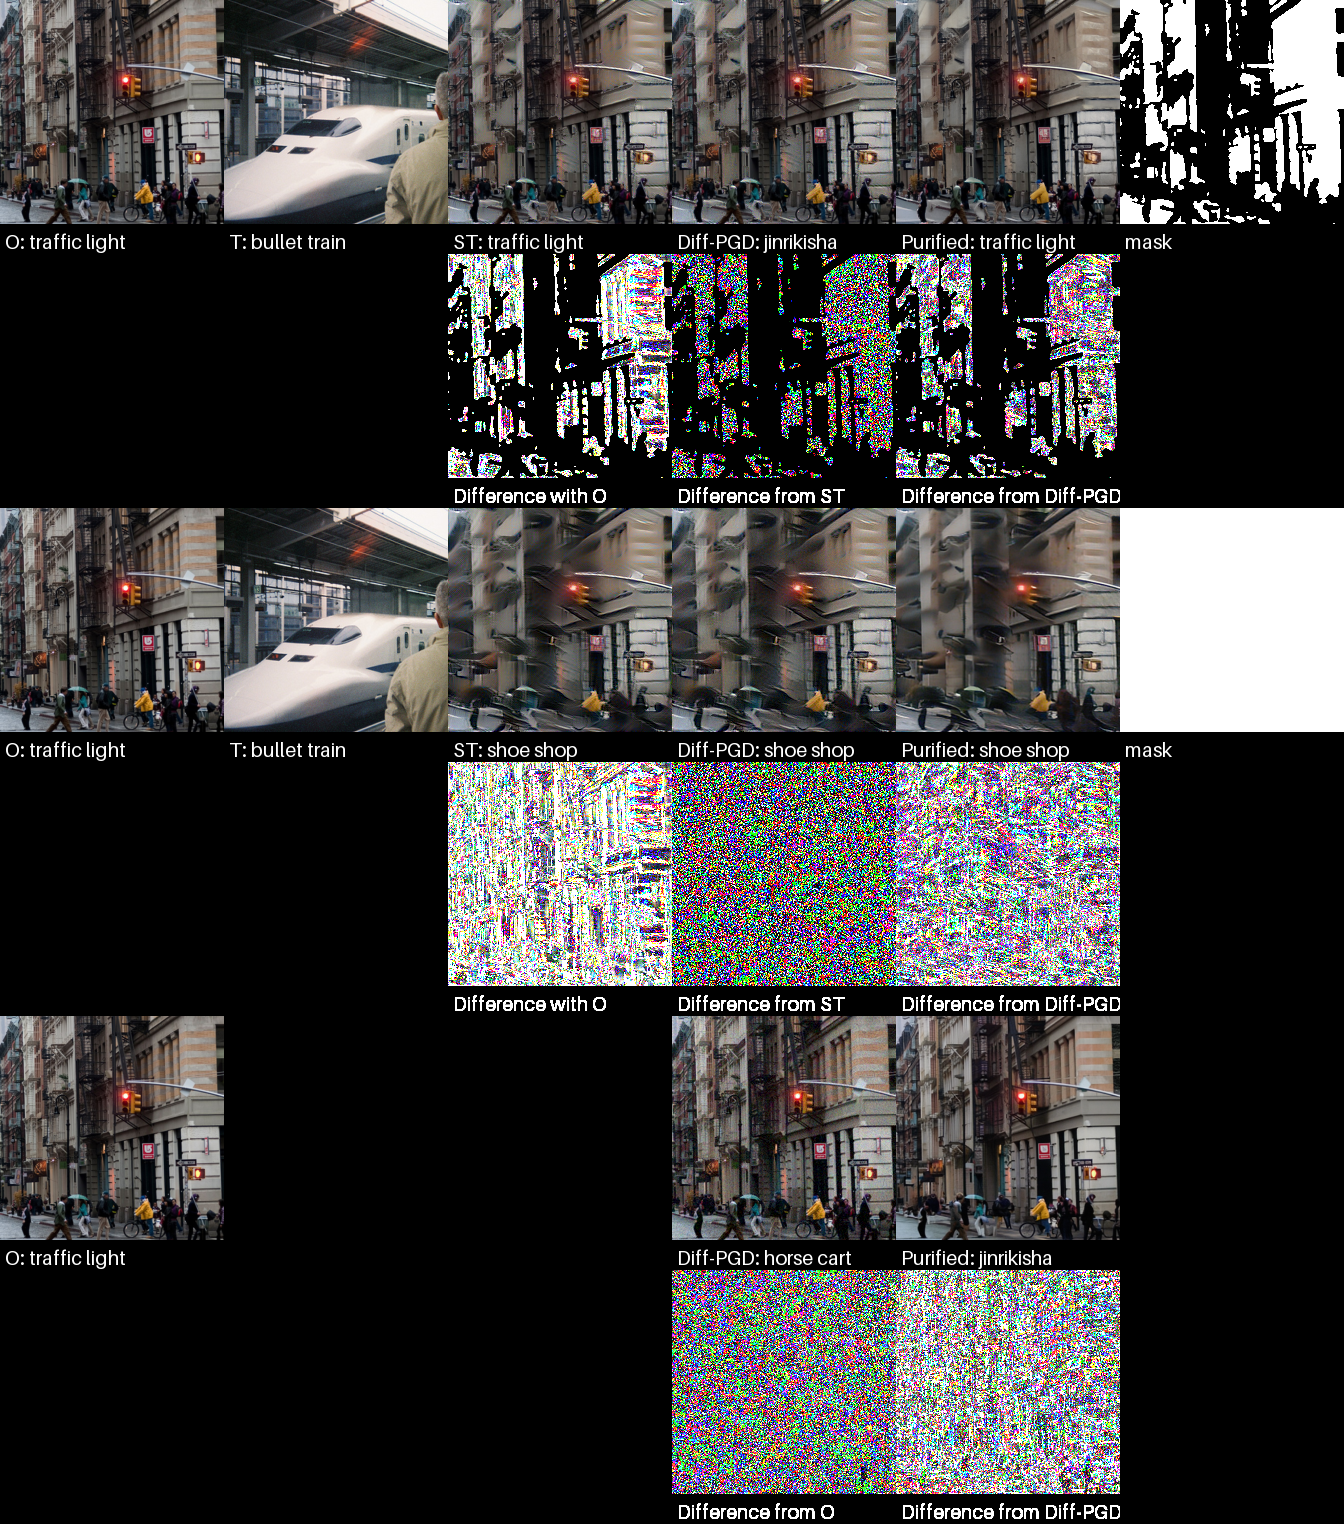
\includegraphics[width=\textwidth]{figures/agoodexample.png}
  \caption{\textbf{Visualization of the different attacks}:} There are 6 rows of images. The first two correspond to a style-based attack with a mask applied. The next 2 rows are the same, except there is no mask. The last 2 rows are a global attack where there is no style image.
  The 6 columns of images are the following: 1: O stands for the original image. 2: T stands for the style image which we try to make the original look more like.
  3: ST is the original image with the style image applied, but no adversarial properties. 4: Has the Diff-PGD algorithm applied. 5. Is the image after going through purification. 6: Is the mask applied.
  \label{fig:attacks}
\end{figure}

\begin{figure}
  \centering
  % The next line would normally be \includegraphics instead.
  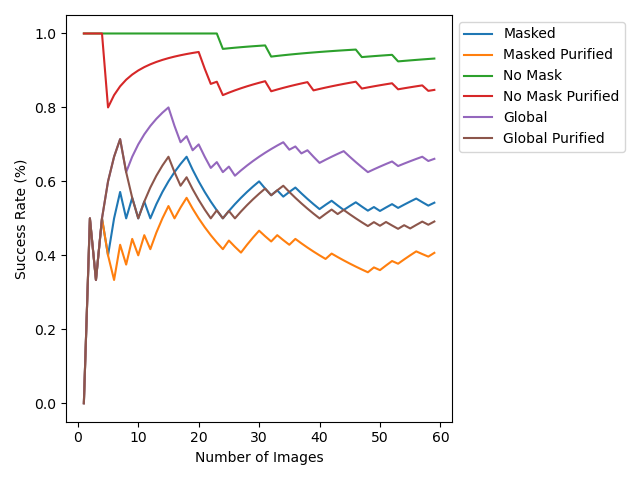
\includegraphics[width=\textwidth]{figures/res_plot.png}
  \caption{\textbf{Plot of the Success Rates}:} We see the best results for applying a style-based attack with no mask. A global attack with no style-image gives the worst results.
  The success rate for purified images is lower than their non-purified versions.
  \label{fig:attacks_plot}
\end{figure}


% \begin{figure}
%   \centering
%   % The next line would normally be \includegraphics instead.
%   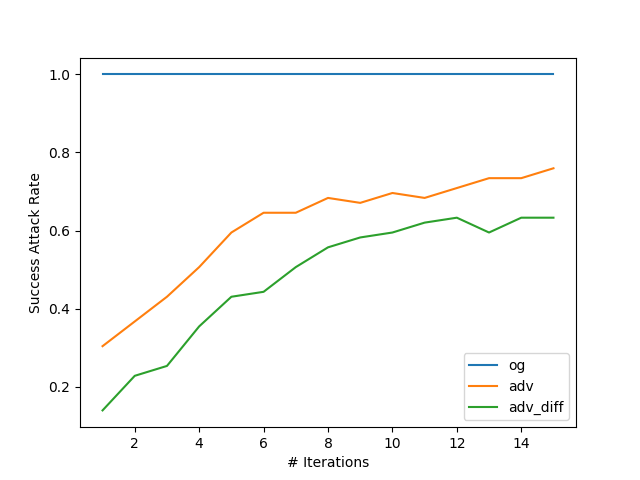
\includegraphics[scale=0.8]{figures/attack_global_gradpass_success_rate.png}

%   \caption{
%     Blue line is success rate of classifying an image not attacked.
%     Orange line is success rate of causing a different classification with Diff-PGD.
%     Green line is success rate of causing a different classification with Diff-PGD after applying sdedit at the end (purification???).
%   }
%   \label{fig:attack_style_success_rate}
% \end{figure}

\subsection{Results beyond original paper}
Often papers don't include enough information to fully specify their experiments, so some additional experimentation may be necessary. For example, it might be the case that batch size was not specified, and so different batch sizes need to be evaluated to reproduce the original results. Include the results of any additional experiments here. Note: this won't be necessary for all reproductions.

\subsubsection{Additional Result 1}

\section{Discussion}

\subsection{Attack Success Rates}
Since the authors have yet to release their code for success rate, we are unsure what caused this difference.
We did use a different dataset than the authors, this could be a possible reason, since for this calculation, we used 78 images per iteration, while the authors used 250.\\
%  however it is unlikely this is the reason, because the authors used pre-trained models, and for the global/digital attacks they only used 250 samples from the ImageNet validation set, while we used 78. \\

% Give your judgement on if your experimental results support the claims of the paper. Discuss the strengths and weaknesses of your approach - perhaps you didn't have time to run all the experiments, or perhaps you did additional experiments that further strengthened the claims in the paper.


\subsection{What was easy}
Running the code from the original authors to generate adversarial samples was fairly easy, since documentation was included in how to run each attack.

The included code had print statements at each iteration, on the speed each iteration was taking, which was helpful in timing how long the model would take to run.
% Give your judgement of what was easy to reproduce. Perhaps the author's code is clearly written and easy to run, so it was easy to verify the majority of original claims. Or, the explanation in the paper was really easy to follow and put into code.

% Be careful not to give sweeping generalizations. Something that is easy for you might be difficult to others. Put what was easy in context and explain why it was easy (e.g. code had extensive API documentation and a lot of examples that matched experiments in papers).

\subsection{What was difficult}
List part of the reproduction study that took more time than you anticipated or you felt were difficult.

Be careful to put your discussion in context. For example, don't say "the maths was difficult to follow", say "the math requires advanced knowledge of calculus to follow".

There was little to no documentation on the inner workings of the code, making it more difficult to understand a lot of the attack parameters, and what they did, however the naming was quite clear for the most part, so this was not too difficult to follow.

The physical-world attack was a lot more difficult to reproduce than we anticipated. AdvCam and AdvPatch both ran fairly quickly, averaging around 2-3s per iteration. However, Diff-PGD averaged around 60s per iteration, which took multiple days to run.
Because of this, instead of running 4000 iterations as was done in the original paper, we only ran 1500 iterations for each image.\\
None of the models were able to perturb the classification of the image, which was likely due to the fact that we did not adjust the scale properly.
This likely means that hyperparameter tuning is very important for physical-world attacks. However, tuning the model is more challenging for Diff-PGD for physical-world attacks, due to how slowly it runs.
Another mistake we made was assuming the the classifier would classify a closed laptop as a laptop, when in reality it classified it as a notebook.
We looked into the ImageNet database, and found that most of the images in both laptop and notebook classes were of open laptops, while we used a closed laptop.
Since the photo's original label was fed into the model, this could have possibly caused problems with the model. \\

\subsection{Communication with original authors}
We did not communicate with the original authors.


\section*{References}

\appendix

\section{Supplementary material} \label{app:info}

\subsection{Physical attacks}

\end{document}
